Several recent papers have used RL training loops,\footnote{Throughout this chapter, the RL training loop runs entirely inside the econometrician's computational model; the agent never interacts with real economic agents or markets but serves as a numerical method for solving the Bellman equation within a structural estimation procedure (Section~\ref{section:language}). There is no execution phase in the usual sense.} namely Q-learning, temporal-difference learning, policy gradient, and actor-critic methods, to solve structural economic models at scales where conventional dynamic programming fails.\footnote{I exclude papers that use neural network function approximation without an RL training mechanism. Inverse reinforcement learning is treated in the sister survey \citep{RustRawat2026}.} Throughout this chapter I adopt a unified notation. An MDP is a tuple $(\mathcal{S}, \mathcal{A}, P, r, \gamma)$ where $\mathcal{S}$ is the state space, $\mathcal{A}$ is the action space, $P(s' | s, a)$ is the transition kernel, $r(s,a)$ is the per-period reward, and $\gamma \in [0,1)$ is the discount factor.\footnote{Several of the papers reviewed here use $\beta$ for the discount factor, following economics convention. I translate all results to $\gamma$ for consistency with the RL literature and the rest of this survey.} A policy $\pi: \mathcal{S} \to \Delta(\mathcal{A})$ maps states to distributions over actions. The value function under $\pi$ is $V^\pi(s) = \mathbb{E}_\pi\left[\sum_{t=0}^\infty \gamma^t r(s_t, a_t) \mid s_0 = s\right]$, and the action-value function is $Q^\pi(s,a) = r(s,a) + \gamma \mathbb{E}_{s' \sim P(\cdot|s,a)}[V^\pi(s')]$. The optimal value function satisfies $V^*(s) = \max_{a \in \mathcal{A}} Q^*(s,a)$.

The canonical structural estimation framework for MDPs was formulated by \citet{rust1994structural}, whose nested fixed-point (NFXP) algorithm embeds the Bellman equation inside a maximum likelihood estimator. The methods reviewed in this chapter replace the inner fixed-point computation with RL-based approximations.

%\subsection{Dynamic Discrete Choice Estimation}

%Dynamic discrete choice (DDC) models are the workhorse of structural empirical economics. An agent in state $s \in \mathcal{S}$ chooses action $a \in \mathcal{A}$ (where $|\mathcal{A}|$ is finite) to maximize
%\begin{equation}
%\mathbb{E}\left[\sum_{t=0}^\infty \gamma^t \left(u(s_t, a_t; \theta) + \varepsilon_t(a_t)\right)\right],
%\end{equation}
%where $u(s,a;\theta) = z(s,a)^\top \theta$ is the deterministic component of per-period utility, $\theta \in \mathbb{R}^d$ collects the structural parameters, and $\varepsilon_t(a)$ is an idiosyncratic shock, typically drawn i.i.d.\ from a Type I extreme value distribution.\footnote{The Type I extreme value (Gumbel) distribution has CDF $F(\varepsilon) = \exp(-\exp(-\varepsilon))$. It yields the logit choice probability $P(a|s) = \exp(V(s,a))/\sum_{a'}\exp(V(s,a'))$, making the model tractable.} The econometrician observes panel data $\{(s_{it}, a_{it})\}_{i=1,\ldots,n}^{t=1,\ldots,T}$ and seeks to recover $\theta$.

%The classical approach of \citet{Rust1987} requires repeated solution of a fixed-point problem (nested fixed-point, or NFXP),\footnote{NFXP solves the likelihood maximization by nesting a Bellman fixed-point computation inside each evaluation of the likelihood function. Each likelihood evaluation requires solving the entire dynamic programming problem, making NFXP computationally expensive.} while the conditional choice probability (CCP) method of \citet{HotzMiller1993} avoids this by exploiting an invertibility result linking choice probabilities to value function differences. Both methods face severe computational challenges when the state space is continuous or high-dimensional. NFXP requires discretization and repeated Bellman iteration, while CCP requires nonparametric estimation of transition densities.

%These computational bottlenecks motivate bringing RL algorithms directly into the DDC estimation pipeline. Two recent papers pursue this approach.

\begin{figure}[t]
\centering
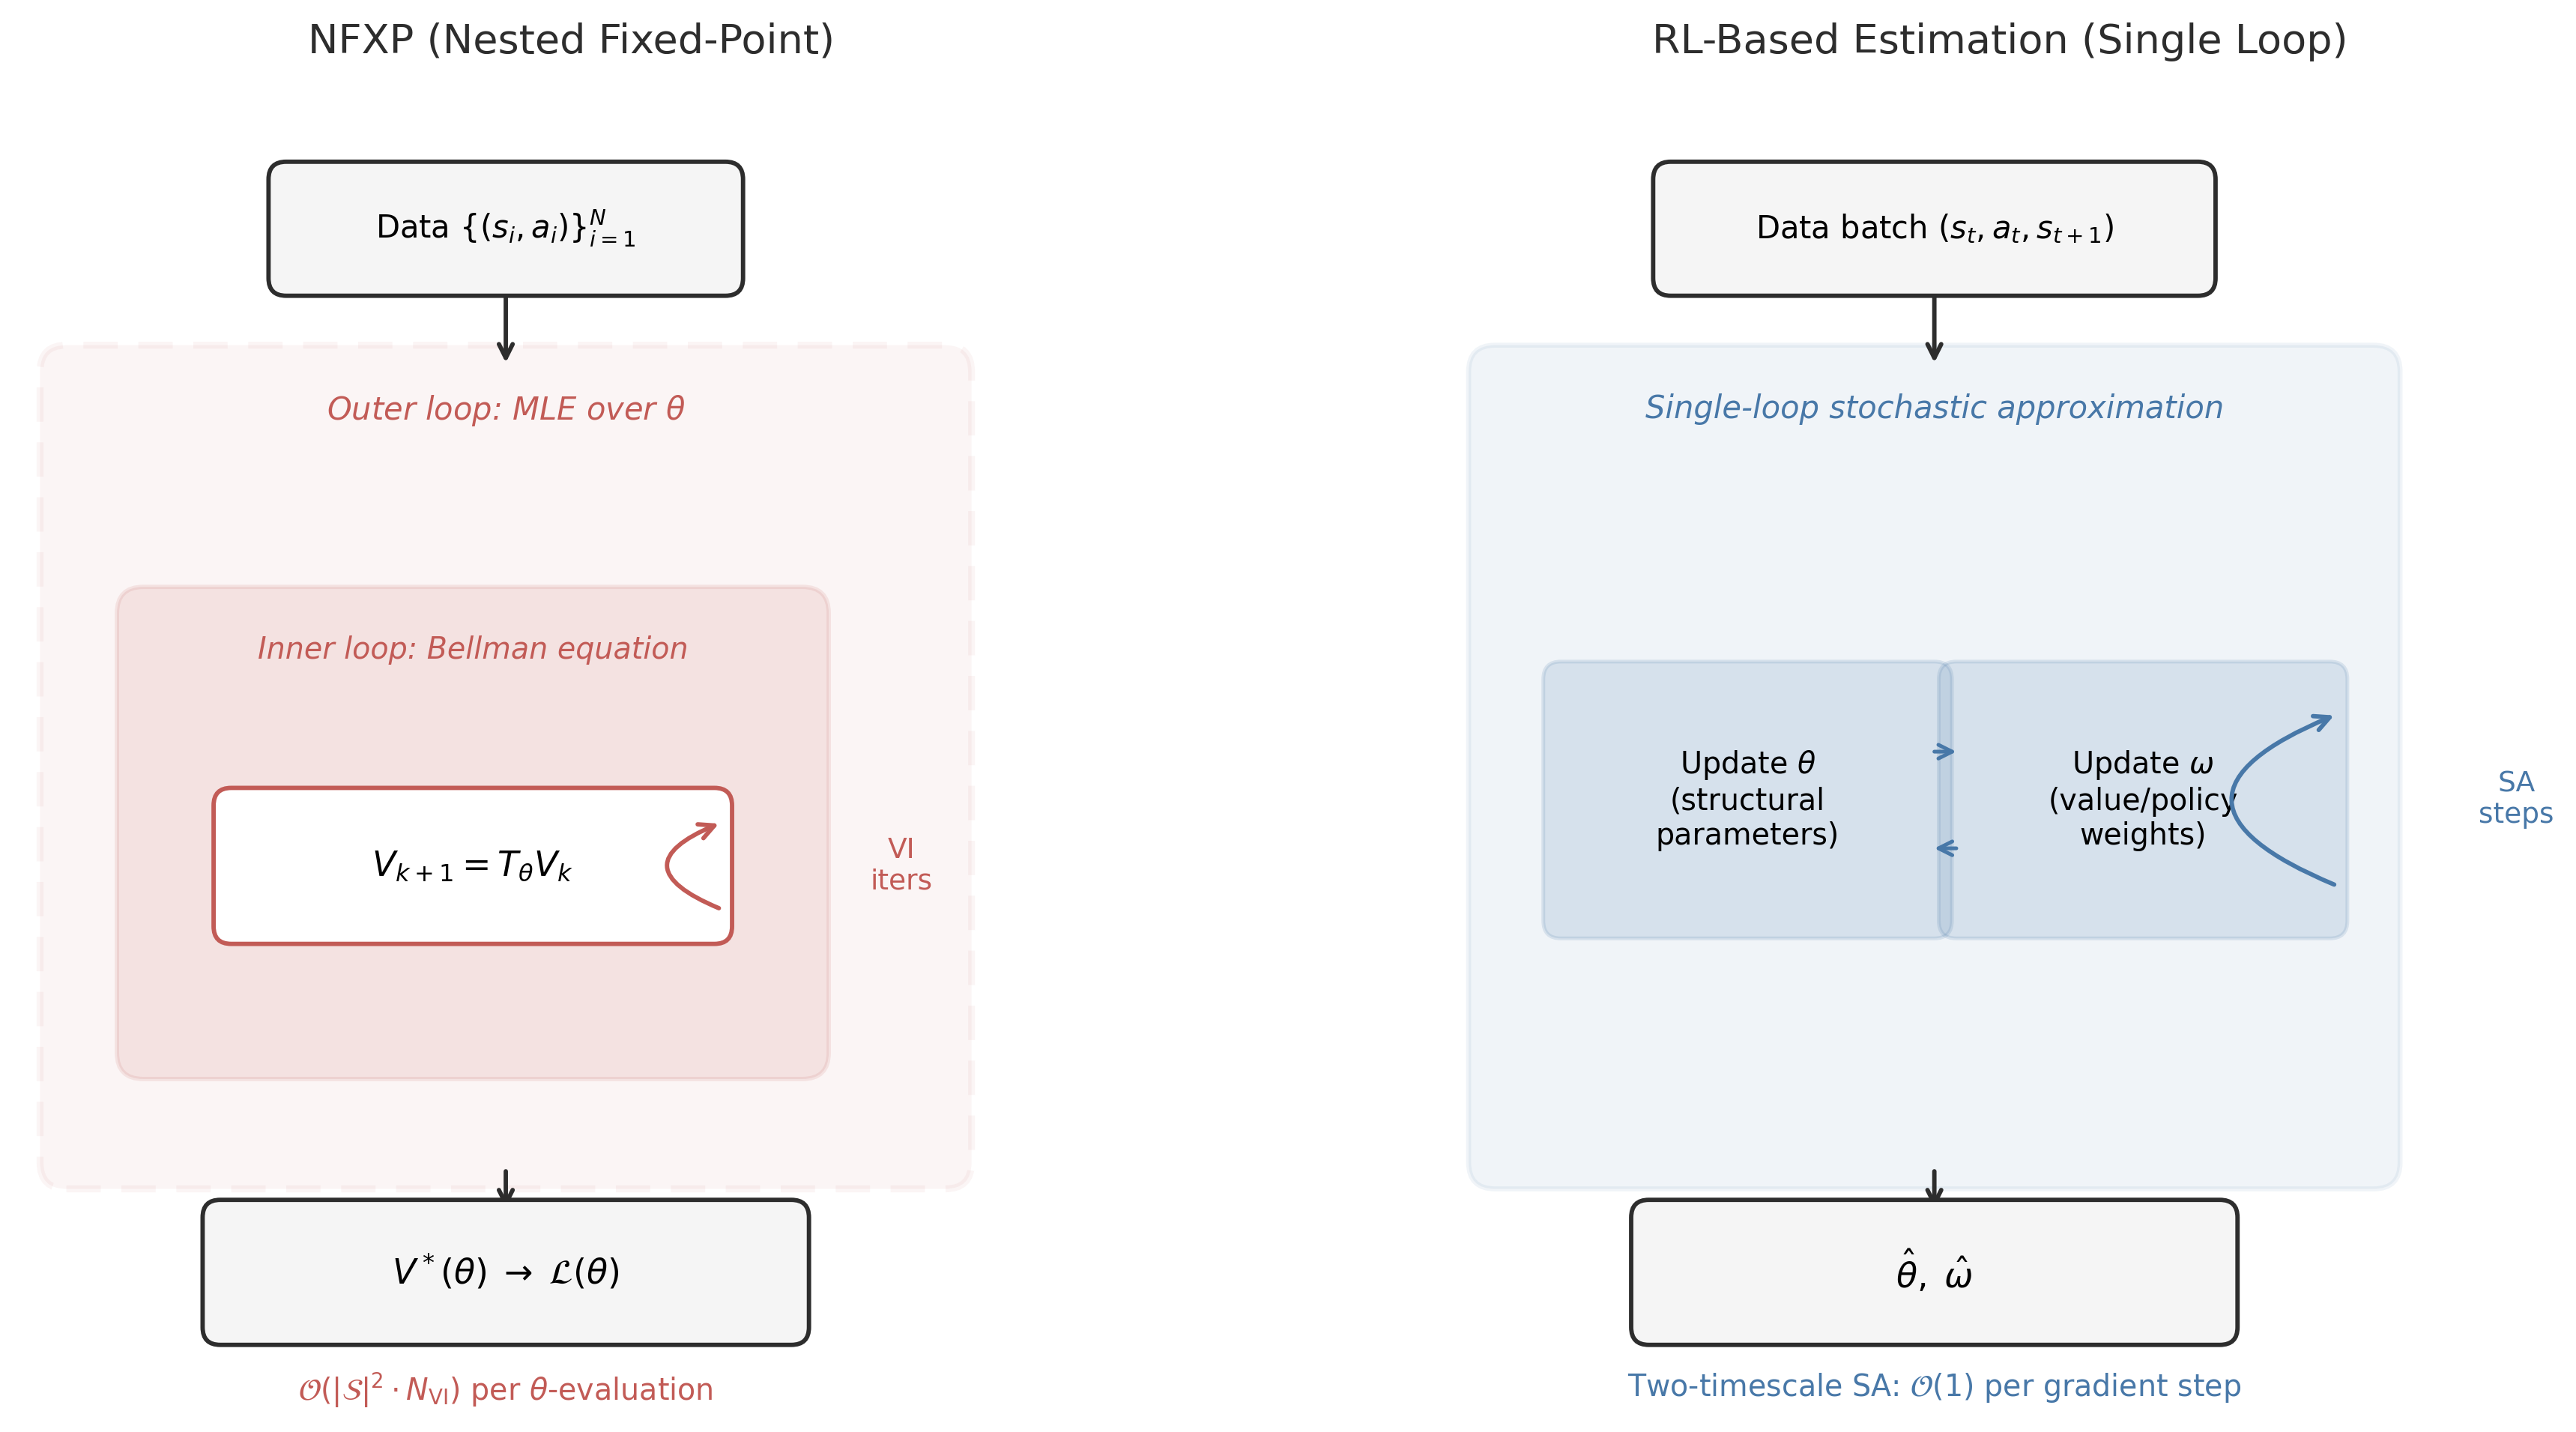
\includegraphics[width=0.85\textwidth]{../ch05_econ_models/sims/estimation_flowcharts.png}
\caption{NFXP versus RL-based structural estimation. Top: the nested fixed-point algorithm evaluates the likelihood by solving the Bellman equation to convergence inside each optimizer step. Bottom: single-loop stochastic approximation updates structural parameters $\theta$ and value/policy weights $\omega$ simultaneously from data batches. The NFXP algorithm is due to \citet{Rust1987}.}
\label{fig:estimation_flowcharts}
\end{figure}

\subsection{Single-Agent Structural Estimation}

\subsubsection{TD Learning for CCP Estimation}

\citet{AdusumilliEckardt2022} adapt temporal-difference (TD) learning to estimate the recursive terms that arise in CCP-based estimation, entirely avoiding specification or estimation of transition densities.

The CCP approach requires computing two functions $h: \mathcal{A} \times \mathcal{S} \to \mathbb{R}^d$ and $g: \mathcal{A} \times \mathcal{S} \to \mathbb{R}$ that solve the recursive equations
\begin{align}
h(a,s) &= z(s,a) + \gamma \, \mathbb{E}[h(a', s') \mid a, s], \label{eq:ae_h}\\
g(a,s) &= e(a,s) + \gamma \, \mathbb{E}[g(a', s') \mid a, s], \label{eq:ae_g}
\end{align}
where $e(a,s) = \gamma_{\text{E}} - \ln P(a|s)$ under logit errors ($\gamma_{\text{E}}$ denoting the Euler constant), and the expectation is over the next-period state-action pair $(s', a')$ given the transition kernel $P(s'|s,a)$ and the observed policy $P(a|s)$. Both $h$ and $g$ satisfy a Bellman-like recursion under the observed (data-generating) policy, not the optimal policy, so standard TD learning applies directly. \citet{AdusumilliEckardt2022} propose two methods.

The first is the linear semi-gradient method.\footnote{The method is called ``semi-gradient'' because it computes the gradient of only the prediction $\phi(a,s)^\top w$ with respect to $w$, not the full TD error including the bootstrap target $\phi(a',s')^\top w$. This avoids differentiating through the target but sacrifices guaranteed convergence in some settings.} Approximate $h(a,s) \approx \phi(a,s)^\top w$ where $\phi: \mathcal{A} \times \mathcal{S} \to \mathbb{R}^p$ is a vector of basis functions (e.g., polynomials in state variables) and $w \in \mathbb{R}^p$ are the weights to be estimated. The TD(0) fixed-point equation is
\begin{equation}
\mathbb{E}\left[\phi(a,s)\left(\phi(a,s) - \gamma \phi(a', s')\right)^\top\right] w = \mathbb{E}\left[\phi(a,s) \, z(s,a)\right]. \label{eq:ae_semigradient}
\end{equation}
The sample analog replaces population expectations with averages over the observed panel.
\begin{equation}
\hat{w} = \left(\frac{1}{n(T-1)} \sum_{i=1}^n \sum_{t=1}^{T-1} \phi_{it}\left(\phi_{it} - \gamma \phi_{i,t+1}\right)^\top\right)^{-1} \left(\frac{1}{n(T-1)} \sum_{i=1}^n \sum_{t=1}^{T-1} \phi_{it} \, z_{it}\right),
\end{equation}
where $\phi_{it} = \phi(a_{it}, s_{it})$ and $z_{it} = z(s_{it}, a_{it})$. This requires inverting a $p \times p$ matrix, where $p$ is the number of basis functions, making computation trivial in most settings. No transition density estimation is needed, since the method uses only observed sequences of current and next-period state-action pairs.

The second method is approximate value iteration (AVI), which iterates the Bellman-like operator using nonparametric regression. At iteration $k$, one constructs pseudo-outcomes
\begin{equation}
Y_{it}^{(k)} = z_{it} + \gamma \, \hat{h}^{(k-1)}(a_{i,t+1}, s_{i,t+1})
\end{equation}
and then fits $\hat{h}^{(k)}$ by regressing $Y_{it}^{(k)}$ on $(a_{it}, s_{it})$ using any machine learning method, including LASSO, random forests, or neural networks.\footnote{\emph{LASSO} \citep{Tibshirani1996} adds an $\ell_1$ penalty to a regression loss, shrinking many coefficients to zero for sparse solutions; \emph{random forests} average many decision trees fit to random subsamples and feature subsets for nonparametric estimation; \emph{neural networks} compose affine transformations with elementwise nonlinearities across multiple layers.} This is the first DDC estimator compatible with arbitrary ML prediction methods, enabling application to very high-dimensional state spaces.

With $\hat{h}$ and $\hat{g}$ in hand, structural parameters are recovered by pseudo-maximum likelihood estimation (PMLE). For continuous state spaces, \citet{AdusumilliEckardt2022} derive a locally robust correction to the PMLE criterion that accounts for the nonparametric first-stage estimation of value terms, restoring $\sqrt{n}$-convergence of $\hat{\theta}$.\footnote{An estimator has $\sqrt{n}$-convergence if its error shrinks at rate $n^{-1/2}$ where $n$ is the sample size. This is the standard parametric rate; slower rates (e.g., $n^{-1/4}$) indicate efficiency loss from nonparametric first stages.} The PMLE score is $m(a,s;\theta,h,g) = \partial_\theta \ln \pi(a,s;\theta,h,g)$, where $\pi$ is the logit choice probability with continuation value $V(a,s) = h(a,s)^\top \theta + g(a,s)$. The naive estimator solves $\mathbb{E}_n[m(a,s;\theta,\hat{h},\hat{g})] = 0$, but with continuous states this moment condition is not orthogonal to the first-stage estimates and converges slower than $\sqrt{n}$. The locally robust moment adds a debiasing correction:
\begin{equation}
\zeta = m(a,s;\theta,h,g) - \lambda(a,s;\theta)\left\{z(s,a)^\top \theta + \gamma \, e(a',s') + \gamma \, V(a',s') - V(a,s)\right\},
\label{eq:ae_robust}
\end{equation}
where $\lambda(a,s;\theta)$ solves a backward recursion that propagates the influence of estimation error through the dynamic structure.\footnote{The term in braces is the temporal-difference error of the continuation value $V$. The adjoint $\lambda$ weights this TD error by its marginal impact on the PMLE score. See Online Appendix B.3 of \citet{AdusumilliEckardt2022} for the derivation.} The corrected estimator $\hat{\theta}_{LR}$ solves $\mathbb{E}_n[\zeta_n] = 0$ and is computationally no harder than the naive PMLE, since the correction is constant in $\theta$.

\begin{theorem}[\citet{AdusumilliEckardt2022}, Theorem 1]
Under regularity conditions, the linear semi-gradient estimator $\hat{h}$ satisfies $\|\hat{h} - h\|_2 = O_P(n^{-1/2}(T-1)^{-1/2})$, where $\|\cdot\|_2$ denotes the $L^2(P)$ norm.\footnote{The $L^2(P)$ norm is $\|f\|_2 = (\int f(x)^2 \, dP(x))^{1/2}$, measuring average squared deviation under the probability measure $P$. This is the natural norm for mean-squared-error analysis.}
\end{theorem}

\begin{theorem}[\citet{AdusumilliEckardt2022}, Theorem 5]
Under regularity conditions on the ML method used in AVI, the locally robust PMLE estimator $\hat{\theta}_{LR}$ satisfies $\sqrt{n}(\hat{\theta}_{LR} - \theta^*) \xrightarrow{d} \mathcal{N}(0, \Sigma)$ for an explicit variance $\Sigma$, even when the state space is continuous.
\end{theorem}

Monte Carlo experiments on a dynamic firm entry model with seven structural parameters and five continuous state variables show that the TD-based estimators achieve a 4- to 11-fold reduction in mean squared error compared to CCP estimators using state-space discretization.

For dynamic discrete games, the method extends naturally. Standard CCP-based estimation of games requires integrating out other players' actions, which becomes intractable with many players or continuous states. TD learning avoids this entirely, since it works directly with the joint empirical distribution of states and their successors. The ``integrating out'' is done implicitly within sample expectations.

\FloatBarrier
\subsection{Engine Replacement MDP: Estimating the Engine's Parameters}
\label{engine:ch05}

\begin{table}[h]
\centering
\caption{Structural parameter recovery in the $+\mathrm{EV}$ Engine Replacement MDP. Population columns use exact choice and transition probabilities. Finite-sample columns report means and standard errors across 20 fixed seeds, with 9,000 transitions per seed.}
\label{tab:engine_estimation}
\small
\begin{tabular}{lrrrr}
\hline
 & \multicolumn{2}{c}{high-mileage keep reward} & \multicolumn{2}{c}{replacement cost} \\
method & population & finite sample & population & finite sample \\
\hline
NFXP & 0.200000 & 0.1993 (0.0038) & 0.500000 & 0.4943 (0.0060) \\
CCP & 0.200000 & 0.1997 (0.0038) & 0.500000 & 0.4934 (0.0059) \\
TD-CCP & 0.200000 & 0.2024 (0.0039) & 0.500000 & 0.4908 (0.0062) \\
\hline
generating value & \multicolumn{2}{c}{0.200000} & \multicolumn{2}{c}{0.500000} \\
\hline
\end{tabular}
\end{table}


The Engine Replacement experiment compares NFXP, CCP, and TD-CCP on the same two structural parameters. Its $+\mathrm{EV}$ variant adds independent Type~I extreme-value shocks with scale $0.4$ to the Engine Replacement MDP. The low-mileage keep reward remains normalized to one, while the high-mileage keep reward and replacement cost have generating values $0.2$ and $0.5$. NFXP recomputes the smoothed Bellman fixed point inside the likelihood \citep{Rust1987}. CCP uses the binary log-odds inversion of \citet{HotzMiller1993}. TD-CCP uses a complete two-state basis to solve sample state-value TD equations, estimates the transition kernel from the same sample, and then applies the same inversion. This finite-state construction is an analogue of the TD approach in \citet{AdusumilliEckardt2022}, not its action-state full-basis estimator.

All three population estimators recover both parameters with maximum absolute error below $10^{-6}$. The finite-sample experiment uses 20 fixed seeds and 9,000 transitions per seed. The mean high-mileage reward estimates range from $0.1993$ to $0.2024$, and the mean replacement-cost estimates range from $0.4908$ to $0.4943$. The reported standard errors are computed across seeds.
\FloatBarrier


\subsubsection{Policy Gradient for DDC Estimation}

\citet{HuYang2025} combine policy gradient methods with the Simulated Method of Moments (SMM) to estimate DDCs, with particular focus on models with unobserved state variables.

The outer loop is SMM.\footnote{SMM \citep{GourierouxMonfort1993} estimates structural parameters by matching moments from simulated data to moments from observed data, avoiding direct evaluation of the likelihood function.} Define a vector of data moments $\mathbf{M}_d$ computed from the observed panel. For candidate structural parameters $\theta$ and transition parameters $\xi$, simulate the model to produce simulated moments $\mathbf{M}_s(\theta, \xi)$. The estimator minimizes
\begin{equation}
(\hat{\theta}, \hat{\xi}) = \arg\min_{\theta, \xi} \left(\mathbf{M}_d - \mathbf{M}_s(\theta, \xi)\right)^\top \mathbf{W} \left(\mathbf{M}_d - \mathbf{M}_s(\theta, \xi)\right), \label{eq:hy_outer}
\end{equation}
where $\mathbf{W}$ is a positive definite weight matrix. Computing $\mathbf{M}_s(\theta, \xi)$ requires solving for the optimal policy under $(\theta, \xi)$, which is the inner-loop problem.

The inner loop parametrizes the choice probability directly as a logistic function of state variables. For a binary choice $J_t \in \{0, 1\}$, the general form is $\Pr(J_t = 1 \mid \boldsymbol{X}_t; \boldsymbol{\gamma}(\theta)) = \text{logistic}(\boldsymbol{X}_t \boldsymbol{\gamma}(\theta))$, where $\boldsymbol{\gamma}(\theta)$ are policy parameters that depend on the structural parameters.\footnote{The linear index can be replaced by higher-order terms of $\boldsymbol{X}_t$ or deep neural networks; the method requires only that the gradient $\nabla_{\boldsymbol{\gamma}} \log \pi_{\boldsymbol{\gamma}}$ has a closed form.} In their application to a Rust bus engine model with unobserved bus condition $S_t^*$, this takes the form
\begin{equation}
\Pr(J_t = 1 \mid X_t, S_t^*, t; \boldsymbol{\gamma}) = \frac{\exp(\gamma_0 + \gamma_1 t + \gamma_2 X_t + \gamma_3 S_t^*)}{1 + \exp(\gamma_0 + \gamma_1 t + \gamma_2 X_t + \gamma_3 S_t^*)}, \label{eq:hy_policy}
\end{equation}
where $t$ enters the index directly to capture time-varying replacement incentives. The policy parameters are updated by REINFORCE-style gradient ascent, applying the policy gradient theorem \citep{Sutton1999}:
\begin{equation}
\nabla_{\boldsymbol{\gamma}} V(\boldsymbol{\gamma}) = \mathbb{E}\left[\sum_{t=0}^{T} \nabla_{\boldsymbol{\gamma}} \log \pi_{\boldsymbol{\gamma}}(J_t \mid X_t, S_t^*, t) \, Q^{\pi_{\boldsymbol{\gamma}}}(X_t, S_t^*, J_t)\right], \label{eq:hy_pg}
\end{equation}
where $Q^{\pi_{\boldsymbol{\gamma}}}$ is the action-value function under the current policy, estimated by Monte Carlo returns from forward-simulated trajectories.

The main contribution is handling unobserved state variables. When state variables are only partially observed, the policy in (\ref{eq:hy_policy}) is parametrized as a function of both $X_t$ and $S_t^*$, and the algorithm forward-simulates trajectories of both observed and unobserved variables.

Building on the nonparametric identification results of \citet{HuShum2012}, the outer-loop SMM targets moments from five consecutive periods of observed data, which suffice to separately identify the structural parameters $\theta$ and transition parameters $\xi$ without requiring the econometrician to observe $S_t^*$. No discretization of continuous unobserved states is needed; the same algorithm handles both discrete and continuous unobserved heterogeneity.

For each candidate $(\theta, \xi)$ in the outer minimization (\ref{eq:hy_outer}), the inner loop runs policy gradient until convergence, producing optimal policy parameters $\boldsymbol{\gamma}^*(\theta, \xi)$. These are used to simulate data and compute $\mathbf{M}_s(\theta, \xi)$.

On an extended Rust bus engine model with a continuous unobserved bus condition following an AR(1) process, estimates of seven structural parameters are centered around their true values across 400 simulations. On a discrete-unobservable variant, the method matches the precision of \citet{ArcidiaconoMiller2011}'s two-step EM algorithm at comparable computation times, though the advantage diminishes as more inner-loop iterations are used for precision.


\subsection{Dynamic Oligopoly and Strategic Interaction}

Dynamic oligopoly models combine game theory and dynamic programming. Firms choose actions strategically while anticipating competitors' strategies, and the state space grows combinatorially in the number of firms.


\subsubsection{Q-Learning in Dynamic Procurement Auctions}

\citet{AskerEtAl2020} develop a computational framework for analyzing dynamic procurement auctions with serially correlated asymmetric information. Their approach builds on the Experience-Based Equilibrium (EBE) concept of \citet{FershtmanPakes2012}, which computes equilibria by simulating industry trajectories and updating strategies toward best responses. EBE evaluates values only on recurrently visited states rather than the full state space, making it feasible for large state spaces. While \citet{FershtmanPakes2012} use a stochastic approximation algorithm to update continuation values from simulated industry trajectories, \citet{AskerEtAl2020} add explicit value-function updates via stochastic approximation.

The model is a repeated first-price sealed-bid auction with two firms. Each firm $i$ maintains a private inventory state $\omega_{i,t}$ (stock of unharvested timber, in their application). The state evolves endogenously, as winning an auction increases inventory while harvesting depletes it. Each firm's private state is not observed by its competitor except at periodic revelation events.

The key computational innovation is the use of Q-learning to compute equilibrium strategies. Each firm $i$ maintains a Q-function $Q_i: \mathcal{S}_i \times \mathcal{A}_i \to \mathbb{R}$, where $\mathcal{S}_i$ encodes firm $i$'s information set (its own inventory, beliefs about the competitor's inventory, public history) and $\mathcal{A}_i$ is its action set (participation decision and bid level). The Q-function satisfies
\begin{equation}
Q_i(s, a) = \mathbb{E}\left[r_i(s, a, a_{-i}) + \gamma \max_{a' \in \mathcal{A}_i} Q_i(s', a') \;\middle|\; s, a\right], \label{eq:asker_bellman}
\end{equation}
where $r_i(s, a, a_{-i})$ is firm $i$'s per-period profit given the state, its own action $a$, and the competitor's action $a_{-i}$, and the expectation is taken over the competitor's strategy and the stochastic transitions.

Firms update Q-values using sample averaging.
\begin{equation}
Q_i(s, a) \leftarrow Q_i(s, a) + \frac{1}{h_k(s,a)}\left[r_i + \gamma \max_{a' \in \mathcal{A}_i} Q_i(s', a') - Q_i(s, a)\right], \label{eq:asker_qupdate}
\end{equation}
where $h_k(s,a)$ is the number of times state-action pair $(s,a)$ has been visited.\footnote{This sample-averaging rule ($\alpha_k = 1/h_k$) is equivalent to maintaining the running mean of observed returns, as distinct from fixed-$\alpha$ Q-learning which gives exponentially decaying weight to older observations. The update is applied for all actions, including counterfactual actions not taken, using the observed state transition.} The equilibrium computation proceeds iteratively, with firms simultaneously updating their Q-functions based on simulated play against each other's current strategies. Strategies are derived from Q-values using an $\varepsilon$-greedy rule or Boltzmann exploration.\footnote{$\varepsilon$-greedy selects the greedy action $\argmax_a Q(s,a)$ with probability $1-\varepsilon$ and a uniformly random action otherwise. Boltzmann exploration selects action $a$ with probability $\propto \exp(Q(s,a)/\tau)$ where $\tau > 0$ is a temperature parameter.}

\citet{AskerEtAl2020} add a boundary consistency condition to the EBE concept that restricts behavior at the boundary of the recurrent state class, reducing the multiplicity of equilibria. Their numerical analysis reveals that information sharing between firms can, through increased precision of beliefs about competitor states, induce firms to spend more time in states where competition is less intense. The dynamic RL-computed equilibrium yields qualitatively different predictions from both static analysis and myopic ($\gamma = 0$) benchmarks. With dynamics, information sharing decreases average bids and increases average profits, while the myopic benchmark shows negligible effects.

The limitation of this approach is the tabular representation; the Q-function is stored as a lookup table over discretized states and actions, restricting applicability to models with moderate state-space dimension.


\subsubsection{TD Learning for Merger Analysis with Innovation}

\citet{Hollenbeck2019} uses RL to solve a dynamic oligopoly model with endogenous mergers, entry, exit, and quality investment. The model extends the Ericson-Pakes framework to study how horizontal mergers affect innovation incentives.

The industry state is $\Omega = (\omega_1, \ldots, \omega_n)$ where $\omega_i \in \{1, \ldots, \omega_{\max}\}$ is firm $i$'s product quality. Firms produce differentiated goods and compete in prices (Bertrand competition with logit demand). In each period, firms simultaneously choose investment levels, entry/exit decisions, and potentially initiate merger negotiations.

Each firm $i$ computes its continuation value $V_i(\Omega)$ from the industry state. Because the state space is the product of all firms' quality levels plus industry structure (number of active firms, recent mergers), exact dynamic programming is infeasible for industries with more than two or three firms. \citet{Hollenbeck2019} instead uses temporal-difference learning to estimate values from simulated industry trajectories.

The value function update for firm $i$ is\footnote{This stochastic approximation update, introduced by \citet{PakesMcGuire1994} for dynamic oligopoly computation, is closely related to temporal-difference learning in the RL literature. The original algorithm uses visit-count averaging ($\alpha_k = 1/k$ where $k$ counts visits to each state) rather than a fixed learning rate.}
\begin{equation}
V_i(\Omega) \leftarrow V_i(\Omega) + \alpha\left[\Pi_i(\Omega, \mathbf{a}) + \gamma V_i(\Omega') - V_i(\Omega)\right], \label{eq:hollenbeck_td}
\end{equation}
where $\Pi_i(\Omega, \mathbf{a})$ denotes firm $i$'s per-period profit given industry state $\Omega$ and the joint action profile $\mathbf{a}$ (investment, entry/exit, merger decisions),\footnote{I use $\Pi_i$ for firm $i$'s per-period profit to avoid confusion with policy $\pi$.} $\gamma$ is the discount factor, and $\Omega'$ is the realized next-period state. The algorithm uses $\varepsilon$-decreasing exploration to prevent convergence to locally suboptimal equilibria.

The equilibrium computation follows the Pakes-McGuire iterative scheme.\footnote{The Pakes-McGuire algorithm \citep{PakesMcGuire1994} computes Markov perfect equilibria by iterating: (1) given current value functions, compute best-response strategies; (2) given strategies, update value functions via simulation. Convergence is not guaranteed but works well in practice.} The algorithm simulates long industry histories, updates each firm's value function via (\ref{eq:hollenbeck_td}), re-derives best-response strategies from updated values, and repeats.

The central finding is that horizontal mergers, while reducing static consumer surplus in the short run, create a strong incentive for entry and investment. Firms enter with negative static profits because the prospect of a lucrative buyout justifies the initial investment. The result is substantially higher long-run innovation and consumer welfare with mergers than without. This finding reverses the standard static antitrust prediction and can only emerge in a dynamic model where firms are forward-looking.

Several recent papers bring RL machinery to dynamic discrete choice and inverse reinforcement learning estimation from other directions. \citet{Kang2025} recast offline inverse RL and DDC estimation as a single empirical risk minimization problem, training the reward function by gradient descent rather than by nested fixed-point iteration. \citet{Khwaja2025} use reinforcement learning to speed up conditional-choice-simulation estimation, \citet{Nguyen2025} estimate high-dimensional DDC models with neural networks, and \citet{Lee2026} apply adversarial IRL to serialized dynamic discrete choice. \citet{DearingBlevins2025} give a convergent sequential pseudo-likelihood estimator for dynamic discrete games.

Two related papers merit brief mention. \citet{LomysMagnolfi2024} develop structural estimation methods for strategic settings where agents use learning algorithms (specifically regret-minimizing rules) rather than playing a fixed equilibrium. They impose an ``asymptotic no-regret'' condition as a minimal rationality requirement and derive identification results for payoff parameters. \citet{Covarrubias2022} uses deep RL to study oligopolistic pricing in a New Keynesian framework, representing firms' pricing policies as neural networks $\pi_\phi(a|s)$. The method uncovers multiple equilibria ranging from competitive to collusive pricing.\footnote{The most prominent example of algorithmic collusion is \citet{Calvano2020}, who showed that independent Q-learning agents in a repeated Bertrand pricing game learn to sustain supra-competitive prices and punish deviators without explicit communication. This result and its implications for competition policy are treated in the companion thesis chapter \citep{Rawat2026collusion}.}


\subsection{Auction Equilibria and Mechanism Design}

Closed-form equilibrium bidding strategies exist only for narrow families of valuation distributions and auction formats, and numerical methods scale poorly with the number of bidders and items.


\subsubsection{RL for Sequential Price Mechanisms}

\citet{BreroEtAl2021} use RL to design optimal sequential price mechanisms (SPMs), a class of indirect auction mechanisms where agents are approached in sequence and offered menus of items at posted prices. SPMs generalize both serial dictatorship and posted-price mechanisms and essentially characterize all strongly obviously strategyproof (SOSP) mechanisms \citep{PyciaAndTroyan2019}.\footnote{A mechanism is strategyproof if truthful reporting is a dominant strategy. It is obviously strategyproof if this dominance is apparent even to boundedly rational agents; strongly obviously strategyproof (SOSP) adds that dominance holds at every information set \citep{PyciaAndTroyan2019}.}

The mechanism design problem is formulated as a partially observable Markov decision process (POMDP).\footnote{In a POMDP, the agent cannot directly observe the full state. It maintains a belief distribution over possible states, updated via Bayes' rule as new observations arrive. This captures the mechanism designer's uncertainty about bidder valuations.} The state at round $t$ includes the set of remaining items $\rho_t^{\text{items}} \subseteq [m]$, remaining agents $\rho_t^{\text{agents}} \subseteq [n]$, the partial allocation $\mathbf{x}_t$, and the agents' (unobserved) valuation functions. The action $a_t = (i_t, \{p_j^t\}_{j \in \rho_{t-1}^{\text{items}}})$ specifies which agent to visit next and what prices to offer. The observation is the agent's purchase decision, from which the mechanism can update beliefs about valuations. The reward is the objective function evaluated at the final allocation:
\begin{equation}
r = g(\mathbf{x}_T, \boldsymbol{\tau}_T; \mathbf{v}), \label{eq:brero_reward}
\end{equation}
where $g$ can be social welfare $\sum_{i} v_i(x_i)$, revenue $\sum_i \tau_i$, or max-min fairness $\min_i v_i(x_i)$.

The theorem below states when adaptive mechanisms outperform static ones.

\begin{theorem}[\citet{BreroEtAl2021}, Propositions 1--4, informal]
Each feature of adaptive mechanisms is necessary for welfare optimality, even in simple settings. Personalized prices are needed with one item and two i.i.d.\ agents (Proposition 1); adaptive prices are needed with two identical items and three i.i.d.\ agents (Proposition 2); adaptive ordering is needed with six agents whose valuations are correlated (Proposition 3); both adaptive prices and ordering are needed with four agents whose valuations are independently but non-identically distributed (Proposition 4).
\end{theorem}

The policy maps from a sufficient statistic of the observation history to actions. \citet{BreroEtAl2021} show that this statistic can be represented compactly. The set of remaining items and agents suffices for independent valuations, while the full allocation matrix is needed for correlated valuations. They train the mechanism policy using Proximal Policy Optimization (PPO),\footnote{Proximal Policy Optimization \citep{Schulman2017} is a policy gradient algorithm that constrains each update to a trust region, preventing large destabilizing policy changes. It is described in Chapter 2.} which handles the discrete action space (agent selection) and continuous action space (price setting) of the POMDP.

Experimental results show that the learned SPMs achieve near-optimal welfare across settings with up to 20 agents and 5 items (with similar results noted for up to 30 of each), significantly outperforming static pricing benchmarks. The improvement is largest when agent valuations are correlated, since adaptive prices allow the mechanism to infer information about remaining agents from earlier purchases.

The limitation is that the POMDP formulation requires knowledge of the prior distribution over valuations, which in practice must be estimated from data. The method also does not scale easily to very large numbers of items due to the combinatorial action space.


\subsubsection{Fitted Policy Iteration for Combinatorial Auctions}

\citet{RavindranathEtAl2024} address revenue-maximizing mechanism design for combinatorial auctions with multiple items and strategic bidders. Their innovation is integrating differentiable auction structure into a fitted policy iteration framework, enabling analytical gradient computation where standard RL methods struggle with high variance.

The mechanism visits agents one at a time in sequence. Each agent $i$, upon being visited, selects a bundle of items from those still available, given posted prices. Valuations are drawn once from distributions $V_i$ and remain fixed throughout the mechanism. Complementarities arise from the structure of the valuation function over bundles, not from dynamic evolution. The MDP state at step $t$ is $s_t = (i_t, S_t)$, where $i_t$ is the current bidder and $S_t$ is the set of remaining items.

The mechanism's policy maps from state to a price vector over available items. The key technical contribution is making the auction clearing differentiable. In a standard auction, the allocation is an argmax over bids (non-differentiable), and payments depend discontinuously on the allocation. \citet{RavindranathEtAl2024} replace the hard bundle selection with a softmax relaxation,\footnote{The softmax relaxation replaces the hard allocation $\argmax_i b_i$ with a soft allocation $\exp(b_i/\tau)/\sum_j \exp(b_j/\tau)$, which is differentiable and approaches the hard allocation as $\tau \to 0$.} enabling analytical gradient computation through the mechanism. The actor loss is the negative expected revenue, and gradients flow directly through the softmax-relaxed allocation and payment rules. The paper explicitly avoids REINFORCE-style estimators, noting that analytical gradients overcome the sample inefficiency and high variance of score-function methods.

The method follows fitted policy iteration \citep{bertsekastsitsiklis1996}, alternating between evaluating the current policy (computing expected revenue) and improving it via gradient ascent on the actor loss. This differs from model-free RL approaches (PPO, SAC) that the paper uses as baselines.

Experiments on settings with additive and combinatorial valuations show that the learned mechanisms achieve up to 13\% higher revenue than item-wise Myerson optimal auctions, with the largest gains in combinatorial settings where bundle complementarities make item-wise pricing suboptimal. Standard RL baselines (PPO, SAC) are also outperformed, confirming the advantage of exploiting differentiable structure.\footnote{DDPG was also tested but found to be unstable. DQN is not applicable to continuous price-setting.}


\subsection{Simulation Study: DDC Estimation at Scale}
\label{sec:ddc_estimation_sim}

The test bed extends the \citet{Rust1987} bus engine replacement model to multiple wear components. In the original formulation a maintenance superintendent observes discretized mileage $m\in\{0,\ldots,M{-}1\}$ and makes a binary keep-or-replace decision, facing running cost $c(s;\theta)=\theta_1 x+\theta_2 x^2$ with $x=m/M$, replacement cost $RC$, and Type~I extreme value additive errors that yield logit conditional choice probabilities. The simulation uses $K$ independent wear components, each evolving in $\{0,\ldots,M{-}1\}$, with aggregate normalized wear $x(s)=\sum_k m_k/M$ entering the same cost function. The state space is $|\mathcal{S}|=M^K$. Increasing $K$ therefore holds the data-generating process fixed while the computational burden grows exponentially.

The experiment compares four estimation methods for $K \in \{1,2,3,4\}$, producing state spaces from 20 to 160,000 states. Panel data consist of $N=500$ agents observed for $T=100$ periods. The methods are NFXP (nested fixed-point MLE), CCP (Hotz-Miller inversion), TD-CCP Linear (semi-gradient TD with polynomial basis), and TD-CCP Neural (approximate value iteration with a two-layer MLP). Both TD-CCP variants follow \citet{AdusumilliEckardt2022}.\footnote{The TD-CCP variants implemented here are simplified relative to \citet{AdusumilliEckardt2022}. We omit the locally robust PMLE correction (Theorem~5 of that paper, the orthogonal moment construction in Section~3.3 and Online Appendix~B.3 that yields $\sqrt{n}$-consistency); the reported point estimates are for the simpler plug-in PMLE and do not inherit the paper's $\sqrt{n}$-convergence guarantee. Empirically, the correction would absorb the first-stage bias from the value-function estimate, narrow the seed-to-seed RMSE, and deliver nominal coverage for confidence intervals built from $\Sigma$ in Theorem~5; the directional scaling story reported below would not change. We also reformulate the bootstrap target by decomposing $EV(s;\theta)$ into $\theta$-linear pieces and learning each piece separately, rather than fitting $h(a,s)$ directly as in the paper; the two are algebraically related under our binary action with one-period reset, but the change is undocumented in the original. Finally, the marketed advantage of TD-CCP that ``no transition density is needed'' is qualified in our implementation: the PMLE step still evaluates $v_0 = -c + \gamma P_{\text{keep}} \widehat{EV}$ using the empirical $P_{\text{keep}}$ assumed known under the Rust convention. A fully density-free variant that replaces $P_{\text{keep}} \widehat{EV}$ by an out-of-sample target average is left for future work.} Each configuration is replicated across 10 seeds with the PyTorch optimizer also seeded. Table~\ref{tab:ddc_estimation} and Figure~\ref{fig:ddc_scaling_time} report means with seed-level standard errors.

\begin{table}[t]
\centering
\caption{DDC estimation results across state-space scales. Rows show method, number of components $K$, state-space size $|\mathcal{S}|$, mean wall-clock time (seconds), RC bias, RC RMSE, and root mean squared error for $\theta_1$ and $\theta_2$. Standard errors in adjacent columns; means over 10 seeds, dashes indicate method failure (sparse state coverage).}
\label{tab:ddc_estimation}
\footnotesize
\begin{tabular}{@{}ll rr cc cc cc cc@{}}
\toprule
 & & & & \multicolumn{2}{c}{RC Bias} & \multicolumn{2}{c}{RC RMSE} & \multicolumn{2}{c}{$\theta_1$ RMSE} & \multicolumn{2}{c}{$\theta_2$ RMSE} \\
\cmidrule(lr){5-6} \cmidrule(lr){7-8} \cmidrule(lr){9-10} \cmidrule(lr){11-12}
Method & K & $|S|$ & Time (s) & Mean & SE & Value & SE & Value & SE & Value & SE \\
\midrule
NFXP & 1 & 20 & 0.2 & +0.053 & 0.027 & 0.097 & 0.015 & 0.307 & 0.055 & 0.495 & 0.111 \\
CCP & 1 & 20 & 0.1 & +0.055 & 0.027 & 0.099 & 0.015 & 0.316 & 0.055 & 0.510 & 0.112 \\
TD-CCP Linear & 1 & 20 & 0.1 & -0.087 & 0.017 & 0.101 & 0.016 & 0.255 & 0.041 & 0.296 & 0.044 \\
TD-CCP Neural & 1 & 20 & 38.4 & +0.054 & 0.026 & 0.094 & 0.013 & 0.260 & 0.054 & 0.423 & 0.082 \\
\midrule
NFXP & 2 & 400 & 0.3 & +0.027 & 0.028 & 0.087 & 0.018 & 0.270 & 0.061 & 0.344 & 0.077 \\
CCP & 2 & 400 & 0.1 & +0.089 & 0.027 & 0.120 & 0.021 & 0.527 & 0.068 & 0.797 & 0.089 \\
TD-CCP Linear & 2 & 400 & 0.1 & -0.171 & 0.021 & 0.182 & 0.021 & 0.131 & 0.027 & 0.888 & 0.060 \\
TD-CCP Neural & 2 & 400 & 32.9 & +0.012 & 0.030 & 0.090 & 0.021 & 0.247 & 0.065 & 0.334 & 0.067 \\
\midrule
NFXP & 3 & 8,000 & 4.4 & +0.011 & 0.014 & 0.044 & 0.009 & 0.236 & 0.046 & 0.364 & 0.081 \\
CCP & 3 & 8,000 & --- & --- & --- & --- & --- & --- & --- & --- & --- \\
TD-CCP Linear & 3 & 8,000 & 0.1 & -0.246 & 0.011 & 0.248 & 0.010 & 0.125 & 0.022 & 1.178 & 0.071 \\
TD-CCP Neural & 3 & 8,000 & 35.9 & +0.007 & 0.017 & 0.051 & 0.009 & 0.215 & 0.050 & 0.318 & 0.081 \\
\midrule
NFXP & 4 & 160,000 & 163.5 & -0.034 & 0.017 & 0.061 & 0.012 & 0.153 & 0.027 & 0.143 & 0.024 \\
CCP & 4 & 160,000 & --- & --- & --- & --- & --- & --- & --- & --- & --- \\
TD-CCP Linear & 4 & 160,000 & 0.2 & -0.328 & 0.014 & 0.331 & 0.014 & 0.226 & 0.028 & 1.103 & 0.027 \\
TD-CCP Neural & 4 & 160,000 & 40.7 & -0.031 & 0.019 & 0.066 & 0.011 & 0.258 & 0.042 & 0.236 & 0.039 \\
\bottomrule
\end{tabular}
\end{table}

\begin{figure}[t]
\centering
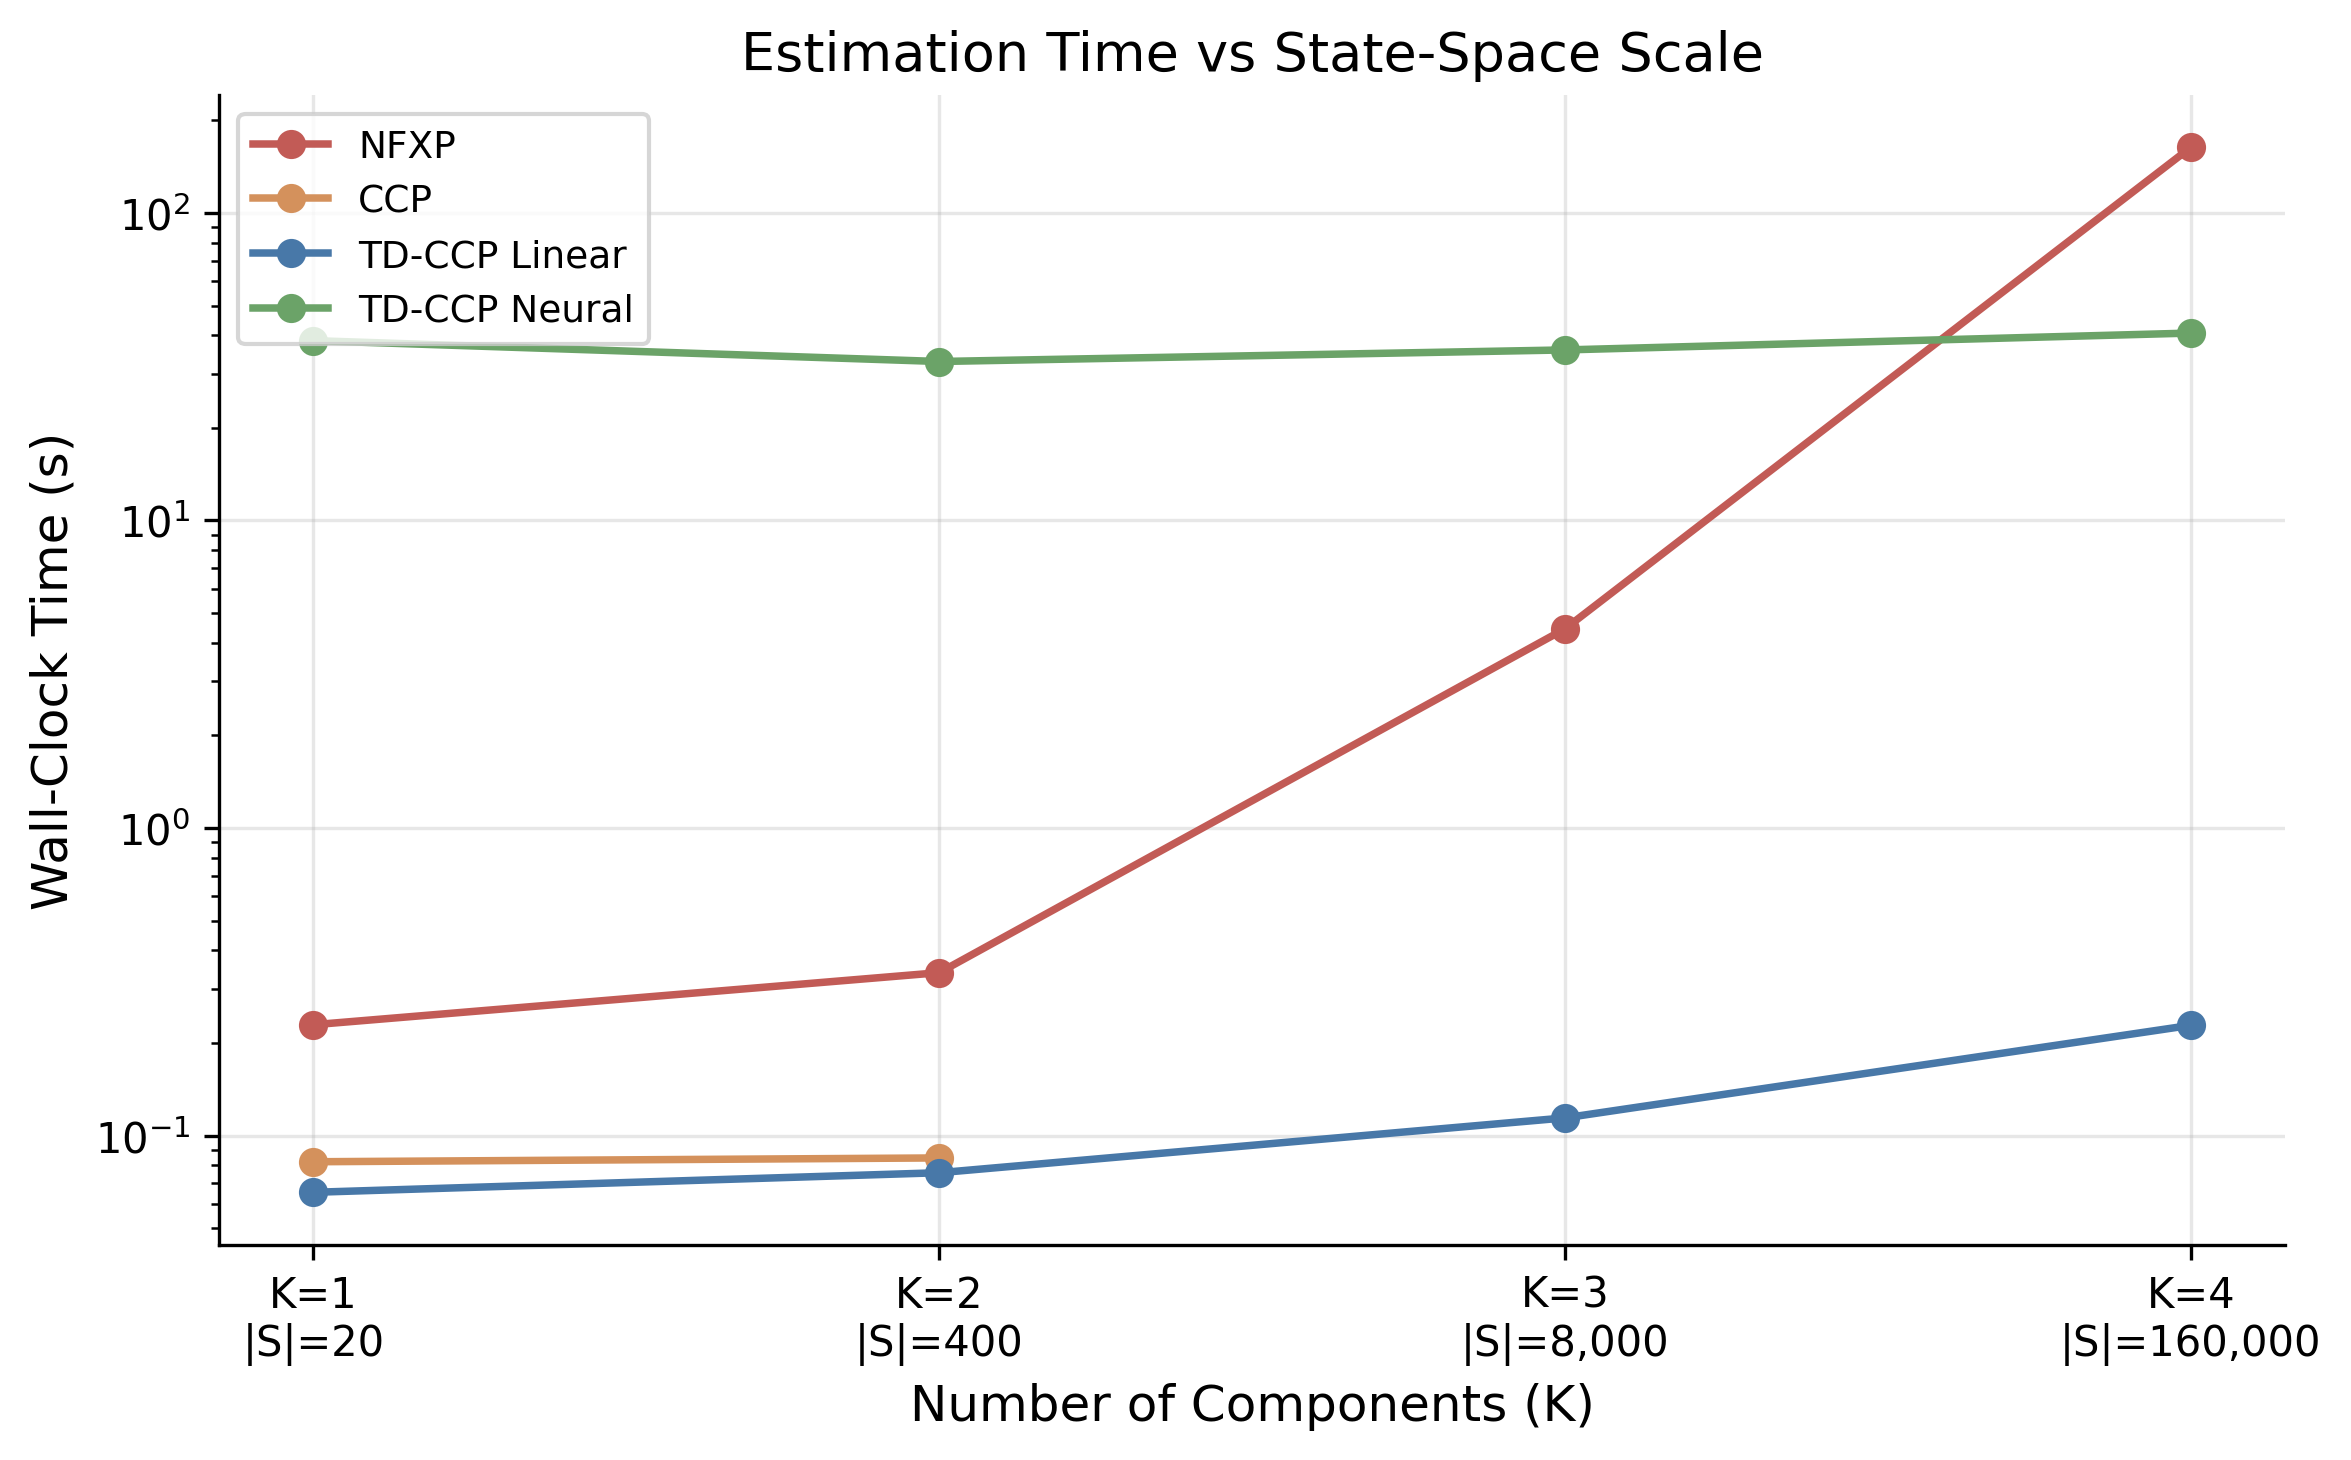
\includegraphics[width=0.85\textwidth]{../ch05_econ_models/sims/nfxp_ccp_td_scaling_time.png}
\caption{Wall-clock estimation time versus state-space scale for the four DDC estimators. Vertical axis is log-scaled. Each point is the mean over 10 seeds.}
\label{fig:ddc_scaling_time}
\end{figure}

Table~\ref{tab:ddc_estimation} reports the numerical comparison. NFXP wall-clock grows by roughly three orders of magnitude across the four scales because each likelihood evaluation repeats value iteration. Sparse state coverage makes CCP infeasible beyond $K{=}2$. TD-CCP Neural maintains near-constant runtime across all $K$ levels with RC RMSE comparable to NFXP, consistent with the AVI approach of \citet{AdusumilliEckardt2022}. At $K{=}4$, TD-CCP Neural has RC RMSE $0.066$ versus $0.061$ for NFXP and wall time $40.7$ seconds versus $163.5$ seconds. This small RMSE difference occurs in the Zurcher-style setup before applying the locally robust correction described above. TD-CCP Linear runs in well under a second at every scale. Its polynomial basis is misspecified at higher $K$, and its RC RMSE rises monotonically with $K$. Figure~\ref{fig:ddc_scaling_time} shows the corresponding runtime curves.
